\documentclass[letterpaper, 12 pt, conference]{ieeeconf} 
\IEEEoverridecommandlockouts                              
\overrideIEEEmargins
\usepackage{setspace}
\usepackage{hyperref}
\hypersetup{
    colorlinks=true,
    urlcolor=blue,
    }

\urlstyle{same}
\usepackage{wrapfig}
\usepackage{multicol}

\usepackage{listings}
\usepackage{color}

\definecolor{dkgreen}{rgb}{0,0.6,0}
\definecolor{gray}{rgb}{0.5,0.5,0.5}
\definecolor{mauve}{rgb}{0.58,0,0.82}

\lstset{frame=tb,
  language=Java,
  aboveskip=0mm,
  belowskip=3mm,
  showstringspaces=false,
  columns=flexible,
  basicstyle={\small\ttfamily},
  numbers=none,
  numberstyle=\tiny\color{gray},
  keywordstyle=\color{blue},
  commentstyle=\color{dkgreen},
  stringstyle=\color{mauve},
  breaklines=true,
  breakatwhitespace=true,
  tabsize=3
}



% The following packages can be found on http:\\www.ctan.org
\usepackage{graphics} % for pdf, bitmapped graphics files
%\usepackage{epsfig} % for postscript graphics files
%\usepackage{mathptmx} % assumes new font selection scheme installed
\usepackage{times} % assumes new font selection scheme installed
%\usepackage{amsmath} % assumes amsmath package installed
%\usepackage{amssymb}  % assumes amsmath package installed
\usepackage{graphicx}

\begin{document}

\thispagestyle{empty}
\pagestyle{empty}

\begin{titlepage}
    \begin{center}
        \vspace*{2.5cm}
 
        \textbf{Feedback Dashboarding Tool}
 
        \vspace{0.5cm}
         Thesis Subtitle
 
         \vfill
        
 
        \textbf{Genevieve Couture}
        200426387 grc839@uregina.ca
 
        \textbf{Payton Gilbertson}
        200248472 gilbertp@uregina.ca
 
        \textbf{Liam Gulak}
        200393578 lgq292@uregina.ca
 
        \textbf{Yunseok Kim}
        200434122 yjk172@uregina.ca
 
        \textbf{Zachary Huber}
        200408160 zeh434@uregina.ca
 
        \vspace{1.5cm}  
        CS 476 Project Report
             
        \vspace{0.8cm}
      
             
        University of Regina\\
        March 21, 2023
             
    \end{center}
 \end{titlepage}


%%%%%%%%%%%%%%%%%%% BODY %%%%%%%%%%%%%%%%%%%%%%%%%%%%%%%%%%%%%%%%%%%%%%%%%%%%%%%%


\doublespacing 
\onecolumn

\section{Problem Definition}
\subsection{Outline the problem requirements and include the application domain and motivations of your project (1 page).}
\linebreak
Business and product owners want meaningful feedback from their customers to assist in their growth and success. It can be difficult to collect this information without onsite hardware and processing the data provided can be a timely task. As with many forms of customer engagement and ratings, customers can be unwilling to participate in traditional methods of feedback if too many steps are required, so the data collected will not be an accurate portrayal of opinions.
\newline


In order to solve this problem, we have created a web application that allows for customers to provide their feedback in a simplistic way, and displays this information for businesses or owners in a way that it simple to understand without the need for onsite hardware. By allowing the customer to interact with a site that is not cumbersome, and can be done from the convenience of their smart phone, many more customers will be willing to submit their thoughts and opinions.
\newline

Our web application is created specifically to benefit business owners or managers who want to monitor the opinions of their clientele in a simplistic way. Based on our previous experiences, these surveys for clientele are often annoying to complete or difficult to find. Often they require typing in a website manually from the back of a receipt which is not worth most people's time. By creating a website that consolidates everything to a simple QR code that can be scanned by a smart phone either posted at the physical location to be rated, or printed on a receipt to be done after the fact. 
\newline

By making surveys more accessible and simple to fill out, more people will be willing to participate, making survey results more accurate. As of now, most people who leave reviews or fill out surveys have extreme opinions which may sway the results in one way or another, so by creating this application, we have hopes that more people will share their opinions making the results much more well rounded.

%%%%%%%%%%%%%%%%%%%%%%%%%%%%%%%%%%%%%%%%%%%%%%%%%%%%%

\newpage    
\section{Application Benefits}
\subsection{What are the benefits of your application when compared to existing systems. Choose two systems only and include their references (2 pages).}
\linebreak
Our application is a simple tool for conducting self-administered surveys. Our users can log into their profiles to view customer feedback to improve their businesses. QR codes can be generated for wide distribution and quick access. SurveyMonkey (\url{https://www.surveymonkey.com/}) and QuestionPro (\url{https://www.questionpro.com/}) are comparable existing systems. Some benefits of our application are that the users can received unlimited number of responses for their surveys without cost and all features to create the surveys are free as well. Our application does not have many templates and complicated tools that may negatively impact loading time. Respondents do not need to create an account to respond to surveys. 

\hfill 

\subsubsection*{Survey Monkey}\hfill 

Survey Monkey is one of the more popular survey platforms as of now. It has lots of different options for different groups of people who may be interested in gaining an insight into people's opinions. With its wide array of available options, it is what many people think of when someone mentions a survey website.
\newline

Survey Monkey's website is very overwhelming to look at on first glance, but after a bit of digging you are able to find a bit of information on the packages available. In the past, they have had a pretty large amount of features for free users, but now their free package is very limited. Currently, their free package only allows for unlimited surveys, but with a restriction of 10 questions each, and only allows for a limited amount of responses. This means that if you want to get information with a large group of people, you would have to create multiples of the same surveys and compile the data together manually.
\newline

Overall, SurveyMonkey is a good tool for users who want to create surveys quickly and easily, but it may not be the best fit for people who want more expansive options for length of survey, and ability to view feedback. The limited free plan and cost may also be a reason for people to choose an alternative.

\break
\subsubsection*{QuestionPro}\hfill

QuestionPro, similar to Survey Monkey, has many different options depending on the customer and type of data they want to collect. It has many of the same options as Survey Monkey has when it comes to questions type, but seems like it's list of features might be more expansive.
\newline

QuestionPro has a very similar home page to Survey Monkey, but made it easier to find the differences between their packages available. This site has many more features available for free users than Survey Monkey, but still has a limit to the amount of questions and responses unless you pay. Rather than limiting to 10 question per survey, QuestionPro allows free users to have up to 100 questions per survey with up to 300 responses which is a very large increase in comparison to Survey Monkey.
\newline

QuestionPro is definitely a powerful tool for creating surveys online, but may be confusing for users with limited technology experiences. The cost for full access is also a restriction for some, but in comparison to Survey Monkey, the free version includes a much larger amount of features and usability.
\newline

Both of these other platforms for similar survey creation to ours lock many features behind a paywall. Our goal to create a very simple survey platform eliminates the confusion from having too many options or limited response allowances to make it more user friendly. We also only have a free option available for all users, so no features are hidden behind a paywall, allowing everyone to have the same experience while using it.

%%%%%%%%%%%%%%%%%%%%%%%%%%%%%%%%%%%%%%%%%%%%%%%%%%%%%

\newpage
\section{Requirements Elicitation and Specification}
\subsection{Functional requirements list (only the ones that you have implemented) for each user role (two exactly). Name each requirement and explain it briefly.}
\linebreak

\textbf{Feedback Gatherer}
\begin{enumerate}
   \item \textbf{Register:} Feedback gatherer creates an account by entering the required information. 
   \item \textbf{Create Survey:} Feedback gatherer creates a survey by entering questions and selecting type of responses.
   \item \textbf{View QR Code:} Feedback gatherer views the generated QR code for the survey.
   \item \textbf{Delete Survey:} Feedback gatherer deletes a survey that is no longer required.
   \item \textbf{View Statistics and Responses:} Feedback gatherer views statistics and responses of a selected survey.
\end{enumerate}

\newline 
\hfill \break

\textbf{Respondent}
\begin{enumerate}
   \item \textbf{Scan QR Code:} Respondent scans the QR code to view the survey.
   \item \textbf{Enter Responses:} Respondent enters responses to the survey questions.
   \item \textbf{Submit Response:} Respondent submits responses to the survey questions.
\end{enumerate}

\newpage

\subsection{For each user role, provide the use case diagram with all the use cases and actors.}

\hfill \break
\begin{figure}[h]
\centering
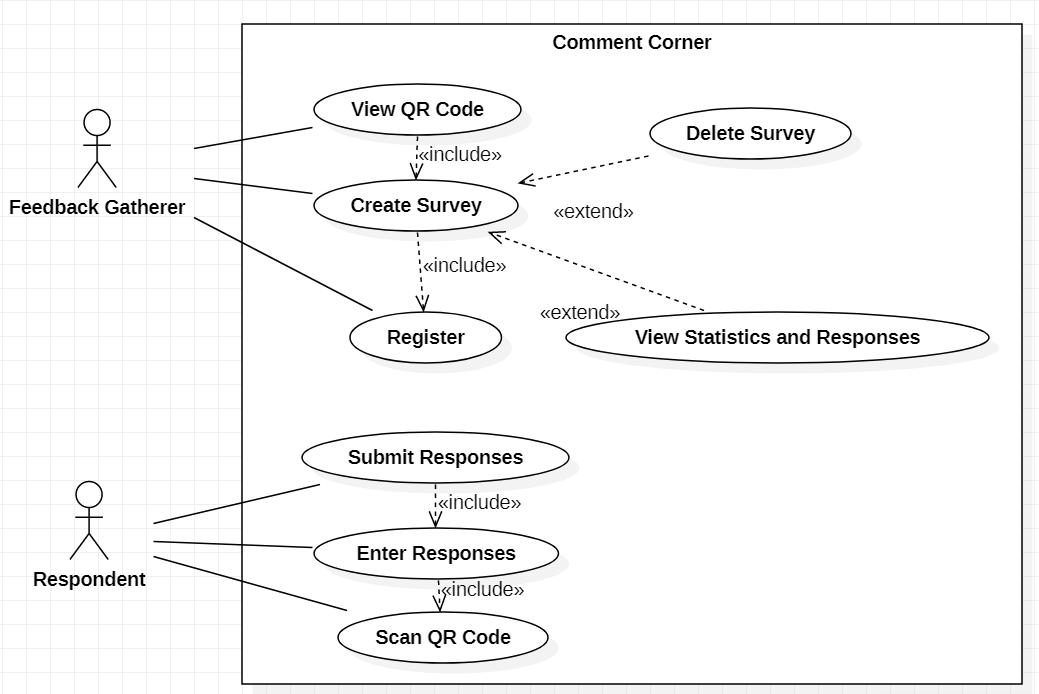
\includegraphics[width=0.70\textwidth]{caseDiagram.png}
\caption{Use Case Diagrams for both the Feedback Gatherer and Respondent}
\end{figure}

\newpage
\subsection{Describe in detail two use cases using the activity diagram. Choose the most complex use cases.}
\begin{enumerate}
    \item The main use case for the feedback gatherer includes: 
    \begin{enumerate}
        \item Creating a survey after registering
        \item Viewing statistics and responses to an existing survey
        \item Viewing the QR code for the survey they created
    \end{enumerate}

    \begin{figure}[h]
        \centering
        \includegraphics[width=0.55\textwidth]{feedbackGatherer2.png}
        \caption{Feedback Gatherer Activity Diagram}
    \end{figure}
\newpage
    \item The main use case for the respondent includes:
    \begin{enumerate}
        \item Scanning the QR code to access the survey previously created by the feedback gatherer
        \item Enter responses to the given survey questions
        \item Submit the completed survey
    \end{enumerate}
    \linebreak

    \begin{figure}[h]
    \centering
    \includegraphics[width=0.70\textwidth]{respondent2.png}
    \caption{Respondent Activity Diagram}
    \end{figure}

\end{enumerate}
\hfill \break
\newpage

\subsection{Software qualities: Correctness, Time-efficiency and Robustness. Include at least two concrete examples for each quality for each user role. The sign-in and sign-up use cases are excluded from the examples.}
\linebreak

\textbf{Correctness:}
\begin{enumerate}
    \item[] Feedback Gatherer:
    \begin{itemize}
        \item A survey correctly displays the questions and answer choices entered by the feedback gatherer during survey creation. 
        \item Accurate statistics for a survey are shown to the feedback gatherer.
    \end{itemize}
    \item[] Respondent:
    \begin{itemize}
        \item Scanning the QR code takes the respondent to the correct survey.
        \item Responses to a survey are saved correctly.
    \end{itemize}
\end{enumerate}
\hfill \break

\textbf{Time Efficiency:}
\begin{enumerate}
    \item[] Feedback Gatherer:
    \begin{itemize}
        \item  When a feedback gatherer creates the survey, the QR code for the survey is created in a timely manner.
        \item When responses to a survey are submitted, they are available to be viewed by the feedback gatherer in a timely manner.
    \end{itemize}
    \item[] Respondent:
    \begin{itemize}
        \item The respondent is taken to the survey in a timely manner after scanning the QR code for a survey.
        \item The respondent is given the submission confirmation in a timely manner after submitting a survey.
    \end{itemize}
\end{enumerate}

\hfill \break
\newpage

\textbf{Robustness:}
\begin{enumerate}
    \item[] Feedback Gatherer:
    \begin{itemize}
        \item  If a feedback gatherer attempts to submit a blank survey, the submission is denied with a warning.
        \item If a feedback gatherer forgets to select a type of answer for a question, submission is denied with a warning.
    \end{itemize}
    \item[] Respondent:
    \begin{itemize}
        \item If a respondent attempts to submit a survey with one or more unanswered questions, the submission is denied and unanswered questions are marked as such.
        \item If a respondent attempts to exit the survey after answering one or more questions, a warning is shown.
    \end{itemize}
\end{enumerate}

%%%%%%%%%%%%%%%%%%%%%%%%%%%%%%%%%%%%%%%%%%%%%%%%%%%%%
\newpage 
\section{Top-level and Low-level Software Design}
\subsection{Provide the MVC architecture according to the selected Web framework. Also, describe at least three benefits of MVC for your application.}
\newline
\hfill

Django uses MVT (Model View Template) architecture which is a variation of the traditional MVC (Model View Controller) architecture. Similar to the MVC, the model in MVT represents the data and business logic. The view in MVT is split into two parts: the template displays the data, and the view handles the user input and interacts with the model to retrieve and manipulate the data. Similarly to the MVC, MVT separates layers and keeps the code organized and maintainable, while also simplifying the view by separating it into two parts. 
\newline

The MVT architecture allows the developer to work on each layer in parallel and then integrate them efficiently. In our project, we used this feature to build and test the three main functions: user authentication process, creation of surveys by the feedback gatherers, and submission of surveys by the respondents. We were able to implement one functionality at a time while working on all of the layers in parallel. One member created the HTML templates while another worked on the models to store the data. Views were then set up followed by finalizing the templates to display the data. Using this method, we were able to develop our web application much faster.
\newline

The MVT architecture allows the developers to make modifications that will not affect the entire model. During development, many changes were required on the templates to enhance the user interface. It was beneficial that the changes in the HTML and CSS only affected the templates and not the entirety of the web application. Many adjustments were also made in the views as well including setting page restrictions for authentication and changing the interactions on the models for submitting data using the forms. Again, the MVT architecture made this process simpler by isolating the modifications.
\newline
\newpage
One major advantage of the Django MVT architecture is the simplified testing process. Since all layers of the application are structurally defined, we were able to test our three main functionalities as we were developing them. For example, for the creation of surveys, the clearly defined structure of the template, model, and view helped us to run tests efficiently. Using an account, we created survey and submitted them and checked the database to verify that the data from the surveys was accurately stored. The clear structure also allowed for efficient debugging and modifications because we knew which template, model, and view were responsible for which functionality.
\newline


\begin{figure}[h]
        \centering
        \includegraphics[width=0.80\textwidth]{mvt.png}
        \caption{MVT Architecture}
    \end{figure}

    \newpage
    
\subsection{Observer and Factory design patterns. Explain in detail the usability of these two patterns for your specific application. Include the complete class diagram for each pattern. Also provide the algorithms corresponding to the pattern’s important methods. For each class, provide the data types of the attributes and prototypes of the methods.}

\textbf{Observer Patterns}

Similar to the MVC architecture, the views in Django’s MVT architecture are the dependent objects while the models are the independent objects. In our application, the observer pattern can be used to manage the relationship between the views and the models by notifying the different views whenever there are changes in the model’s data. This can be useful since there are multiple views that are affected by the changes in the data. For example, when a user adds or deletes a survey, this change would be reflected in the survey model. All of the views related to this model would be notified of these changes. The user profile template would display the addition or the deletion of a survey while a new survey page template would be created or deleted. The observer model can be useful in maintaining consistency between the related objects and keeping them up to date. 
\newline
\clearpage

\begin{figure}[h]
        \centering
        \includegraphics[width=0.75\textwidth]{AuthUserClass.png}
        \caption{AuthUser Class}
\end{figure}

\begin{lstlisting}
AuthUser Data Algorithm

interface class Subject
{
	protected observerList: array of Observer
	public void register(Observer)
	public void unregister(Observer)
	public void notify()
}
class AuthUser Data implements Subject
{
	private int is_superuser, is_staff, is_active
	private string password, last_login, username, first_name, last_name, email, date_joined
	public void register(Observer obs)
		observerList.add(obs)
	public void unregister(Observer obs)
		observerList.delete(obs)
	public void notify()
		for each obs in observerList
			obs.update(is_superuser, is_staff, is_active, password, last_login, username, first_name, last_name, email, date_joined)
	public void sendAuthUser() //calls notify()
	public type getState()
		return subjectState
}


interface class Observer
{
	public void update(int, int, int, string, string, string, string, string, string, string)
}
class authUser implement Observer
{
	private int is_superuser, is_staff, is_active
	private string password, last_login, username, first_name, last_name, email, date_joined
	public void update(int is_superuserX, int is_staffX, int is_activeX, astring passwordX, string last_loginX, string usernameX, string first_nameX, string last_nameX, string emailX, string date_joinedX)
	{
		is_superuser = is_superuserX
		is_staff = is_staffX
		is_active = is_activeX
		password = passwordX
		last_login = last_loginX
		username = usernameX
		first_name = first_nameX
		last_name = last_nameX
		email = emailX
		date_joined = date_joinedX
		displayView()
	}
	public void displayView()
}
\end{lstlisting}
\clearpage


\begin{figure}[h]
        \centering
        \includegraphics[width=0.85\textwidth]{ResponsesData.png}
        \caption{Responses Data}
    \end{figure}

\begin{lstlisting}
Responses Data Algorithm

interface class Subject
{
	protected observerList: array of Observer
	public void register(Observer)
	public void unregister(Observer)
	public void notify()
}
class ResponsesData implements Subject
{
	private int response_id, form_id, user_id
	private string response_json, created_at, updated_at
	public void register(Observer obs)
		observerList.add(obs)
	public void unregister(Observer obs)
		observerList.delete(obs)
	public void notify()
		for each obs in observerList
			obs.update(response_id, form_id, user_id, response_json, created_at, updated_at)
	public void sendResponse() //calls notify()
	public type getState()
		return subjectState
}


interface class Observer
{
	public void update(int, int, int, string, string, string)
}
class deleteForm implement Observer
{
	private int response_id, form_id, user_id
	private string response_json, created_at, updated_at
	public void update(int response_idX, int form_idX, int user_idX, string response_jsonX, string created_atX, string updated_atX)
	{
		response_id = response_idX
		form_id = form_idX
		user_id = user_idX
		response_json = response_jsonX
		created_at = created_atX
		updated_at = updated_atX
		displayView()
	}
	public void displayView()
}
class saveResponses implement Observer
{
	private int response_id, form_id, user_id
	private string response_json, created_at, updated_at
	public void update(int response_idX, int form_idX, int user_idX, string response_jsonX, string created_atX, string updated_atX)
	{
		response_id = response_idX
		form_id = form_idX
		user_id = user_idX
		response_json = response_jsonX
		created_at = created_atX
		updated_at = updated_atX
		displayView()
	}
	public void displayView()
}
class results implement Observer
{
	private int response_id, form_id, user_id
	private string response_json, created_at, updated_at
	public void update(int response_idX, int form_idX, int user_idX, string response_jsonX, string created_atX, string updated_atX)
	{
		response_id = response_idX
		form_id = form_idX
		user_id = user_idX
		response_json = response_jsonX
		created_at = created_atX
		updated_at = updated_atX
		displayView()
	}
	public void displayView()
}
\end{lstlisting}

\clearpage
\begin{figure}[h]
        \centering
        \includegraphics[width=0.85\textwidth]{FormsData.png}
        \caption{Forms Data}
    \end{figure}

\begin{lstlisting}
Forms in Projects Application Algorithm

interface class Subject
{
	protected observerList: array of Observer
	public void register(Observer)
	public void unregister(Observer)
	public void notify()
}
class FormsData implements Subject
{
	private int form_id, user_id, is_active
	private string title, description, created_at, updated_at, form_json
	public void register(Observer obs)
		observerList.add(obs)
	public void unregister(Observer obs)
		observerList.delete(obs)
	public void notify()
		for each obs in observerList
			obs.update(form_id, user_id, is_active, title, description, created_at, updated_at, form_json)
	public void sendForms() //calls notify()
	public type getState()
		return subjectState
}


interface class Observer
{
	public void update(int, int, int, string, string, string, string, string)	
}
class survey implement Observer
{
	private int form_id, user_id, is_active
	private string title, description, created_at, updated_at, form_json
	public void update(int form_idX, int user_idX, int is_activeX, string titleX, string descriptionX, string created_atX, string updated_atX, string form_jsonX)
	{
		form_id = form_idX
		user_id = user_idX
		is_active = is_activeX
		title = titleX
		description = descriptionX
		created_at = created_atX
		updated_at = updated_atX
		form_json = formjsonX
		displayView()
	}
	public void displayView()
}
class saveFormEditor implement Observer
{
	private int form_id, user_id, is_active
	private string title, description, created_at, updated_at, form_json
	public void update(int form_idX, int user_idX, int is_activeX, string titleX, string descriptionX, string created_atX, string updated_atX, string form_jsonX)
	{
		form_id = form_idX
		user_id = user_idX
		is_active = is_activeX
		title = titleX
		description = descriptionX
		created_at = created_atX
		updated_at = updated_atX
		form_json = formjsonX
		displayView()
	}
	public void displayView()
}
class deleteForm implement Observer
{
	private int form_id, user_id, is_active
	private string title, description, created_at, updated_at, form_json
	public void update(int form_idX, int user_idX, int is_activeX, string titleX, string descriptionX, string created_atX, string updated_atX, string form_jsonX)
	{
		form_id = form_idX
		user_id = user_idX
		is_active = is_activeX
		title = titleX
		description = descriptionX
		created_at = created_atX
		updated_at = updated_atX
		form_json = formjsonX
		displayView()
	}
	public void displayView()
}
class results implement Observer
{
	private int form_id, user_id, is_active
	private string title, description, created_at, updated_at, form_json
	public void update(int form_idX, int user_idX, int is_activeX, string titleX, string descriptionX, string created_atX, string updated_atX, string form_jsonX)
	{
		form_id = form_idX
		user_id = user_idX
		is_active = is_activeX
		title = titleX
		description = descriptionX
		created_at = created_atX
		updated_at = updated_atX
		form_json = formjsonX
		displayView()
	}
	public void displayView()
}
\end{lstlisting}


\clearpage
\textbf{Factory Patterns}

In our application, the factory design pattern can be used to store the family of objects in one class and to keep the code of building the objects hidden from the clients. For example, a factory class can be used for the creation of surveys, which is a family of related objects. The factory class would be the centralized class that creates a family of different surveys. This results in consistent products for all clients while having a highly maintainable program with no duplication of code. The factory class would return a survey depending on the questions and the type of answers selected by the client. The factory design pattern is useful for our application because we have many users that need the same family of objects which is the survey.

\linebreak
    \hfill \break
\clearpage
\begin{figure}[h]
        \centering
        \includegraphics[width=0.75\textwidth]{FactoryAuthUser.png}
        \caption{AuthUser Class}
\end{figure}

\begin{lstlisting}
class AuthUserSimpleFactory
{
	public AuthUser createAuthUser(string type)
	if (type == "AuthUser1") return new AuthUser1()
	else if (type == "AuthUser2") return new AuthUser2()
		.
		.
		.
		else if (type == "AuthUserN") return new AuthUserN() 
}
class User1
{
	private AuthUserSimpleFactory sfo
	public AuthUser requestAuthUser(string type)
	{
		AuthUser myAuthUser = sfo.createAuthUser(type)
		myAuthUser.register()
		return myAuthUser
	{	
}
.
.
.
class UserN
{
	private AuthUserSimpleFactory sfo
	public AuthUser requestAuthUser(string type)
	{
		AuthUser myAuthUser = sfo.createAuthUser(type)
		myAuthUser.register()
		return myAuthUser
	{	
}
abstract class AuthUser
{
	protected password, last_login, username, first_name, last_name, email, date_joined: string
	protected is_superuser, is_staff, is_active: int
	public void register()	
	{ }
}
class AuthUser1 extends AuthUser
{
	AuthUser1() //assign values entered by the user during registration
	{
		password = "password1"
		last_login = "last_login1"
		username = "username1"
		first_name = "first_name1"
		last_name = "last_name1"
		email = "email1"
		date_joined = "date_joined1"
		is_superuser = 0
		is_staff = 0
		is_active = 1
	}
	public void register()
	{ }
}
.
.
.
class AuthUserN extends AuthUser
{
	AuthUserN() //assign user entered values during registration
	{
		password = "passwordN"
		last_login = "last_loginN"
		username = "usernameN"
		first_name = "first_nameN"
		last_name = "last_nameN"
		email = "emailN"
		date_joined = "date_joinedN"
		is_superuser = 0
		is_staff = 0
		is_active = 1
	}
	public void register()
	{ }
}
\end{lstlisting}

\clearpage
\begin{figure}[h]
        \centering
        \includegraphics[width=0.8\textwidth]{FactoryForms.png}
        \caption{Forms Class}
\end{figure}

\begin{lstlisting}
class FormsSimpleFactory
{
	public forms createForms(string type)
	if (type == "Forms1") return new Forms1()
	else if (type == "Forms2") return new Forms2()
	.
	.
	.
		else if (type == "FormsN") return new FormsN()
}
class User1
{
	private FormsSimpleFactory sfo
	public forms submitForms(string type)
		{
			forms myForms = sfo.createForms(type)
			myForms.saveFormEditor()
			return myForms
		}
}
.
.
.
class UserN
{
	private FormsSimpleFactory sfo
	public forms submitForms(string type)
		{
			forms myForms = sfo.createForms(type)
			myForms.saveFormEditor()
			return myForms
		}
}
abstract class forms
{
	protected form_id, user_id, is_active: int
	protected title, description, created_at, updated_at, form_json: string
	public void saveFormEditor()
	{ }
}
class forms1 extends forms
{
	Forms1() //assign user entered values during form creation
	{
		form_id = 1
		user_id = 1
		is_active = 1
		title = "title1"
		description = "description1"
		created_at = "created_at1"
		updated_at = "updated_at1"
		form_json = "form_json1"
	}
	public void saveFormEditor()
	{ }
}
.
.
.
class formsN extends forms
{
	FormsN() //assign user entered values during form creation
	{
		form_id = N
		user_id = N
		is_active = N
		title = "title1"
		description = "description1"
		created_at = "created_at1"
		updated_at = "updated_at1"
		form_json = "form_json1"
	}
	public void saveFormEditor()
	{ }
}
\end{lstlisting}

\clearpage
\begin{figure}[h]
        \centering
        \includegraphics[width=0.8\textwidth]{FactoryResponses.png}
        \caption{Responses Class}
\end{figure}

\begin{lstlisting}
class ResponsesSimpleFactory
{
	public responses createResponses(string type)
	if (type == "Responses1") return new Responses1()
	else if (type == "Responses2") return new Responses2()
	.
	.
	.
		else if (type == "ResponsesN") return new ResponsesN()
}
class User1
{
	private ResponsesSimpleFactory sfo
	public responses createResponses(string type)
	{
		responses myResponses = sfo.createResponses(type)
		myResponses.saveResponses()
		return myResponses
	}
}
.
.
.
class UserN
{
	private ResponsesSimpleFactory sfo
	public responses createResponses(string type)
	{
		responses myResponses = sfo.createResponses(type)
		myResponses.saveResponses()
		return myResponses
	}
}
abstract class responses
{
	protected response_id, form_id, user_id: int
	protected response_json, created_at, updated_at: string
	public void saveResponses()
	{ }
}
class Responses1 extends responses
{
	Responses1() //assign values entered by the user during response creation
	{
		response_id = 1
		form_id = 1
		user_id = 1
		response_json = "response_json1"
		created_at = "created_at1"
		updated_at = "updated_at1"
	}
	public void saveResponses()
	{ }	
}
.
.
.
class ResponsesN extends responses
{
	ResponsesN() //assign values entered by the user during response creation
	{
		response_id = N
		form_id = N
		user_id = N
		response_json = "response_jsonN"
		created_at = "created_atN"
		updated_at = "updated_atN"
	}
	public void saveResponses()
	{ }	
}
\end{lstlisting}

\newpage
\subsection{Provide the class diagram of the whole system by incorporating the two design patterns.}

\begin{figure}[h]
        \centering
        \includegraphics[width=\textwidth]{entireClassDiagram.png}
        \caption{Whole System Class Diagram}
\end{figure}

\linebreak
    \hfill \break
\newpage
%%%%%%%%%%%%%%%%%%%%%%%%%%%%%%%%%%%%%%%%%%%%%%%%%%%%%


\section{Software Construction}
\subsection{Submit the screenshot of the entire structure of the code within the web framework.}

\singlespacing
\begin{lstlisting}
    ├───dLocal
│   └───dLocal
│       │   db.sqlite3
│       │   manage.py
│       │   models.py
│       │
│       ├───CS476P
│       │   │   asgi.py
│       │   │   settings.py
│       │   │   urls.py
│       │   │   wsgi.py
│       │   │   __init__.py
│       │   │
│       │   └───__pycache__
│       │           settings.cpython-310.pyc
│       │           settings.cpython-311.pyc
│       │           urls.cpython-310.pyc
│       │           urls.cpython-311.pyc
│       │           wsgi.cpython-310.pyc
│       │           wsgi.cpython-311.pyc
│       │           __init__.cpython-310.pyc
│       │           __init__.cpython-311.pyc
│       │
│       ├───projects
│       │   │   admin.py
│       │   │   apps.py
│       │   │   models.py
│       │   │   tests.py
│       │   │   urls.py
│       │   │   views.py
│       │   │   __init__.py
│       │   │
│       │   ├───migrations
│       │   │   │   0001_initial.py
│       │   │   │   0002_tag_project_vote_ratio_project_vote_total_review_and_more.py
│       │   │   │   0003_form_project_featured_image_response.py
│       │   │   │   0004_project_owner.py
│       │   │   │   0005_alter_form_created.py
│       │   │   │   0005_rename_created_form_created_at_remove_form_id_and_more.py
│       │   │   │   0006_forms_projectsform.py
│       │   │   │   0006_rename_created_response_created_at_and_more.py
│       │   │   │   0007_merge_20230319_1823.py
│       │   │   │   __init__.py
│       │   │   │
│       │   │   └───__pycache__
│       │   │           0001_initial.cpython-310.pyc
│       │   │           0001_initial.cpython-311.pyc
│       │   │           0002_tag_project_vote_ratio_project_vote_total_review_and_more.cpython-310.pyc
│       │   │           0002_tag_project_vote_ratio_project_vote_total_review_and_more.cpython-311.pyc
│       │   │           0003_form_project_featured_image_response.cpython-310.pyc
│       │   │           0003_form_project_featured_image_response.cpython-311.pyc
│       │   │           0004_project_owner.cpython-310.pyc
│       │   │           0004_project_owner.cpython-311.pyc
│       │   │           0005_alter_form_created.cpython-310.pyc
│       │   │           0005_rename_created_form_created_at_remove_form_id_and_more.cpython-310.pyc
│       │   │           0006_forms_projectsform.cpython-310.pyc
│       │   │           0006_rename_created_response_created_at_and_more.cpython-310.pyc
│       │   │           0007_merge_20230319_1823.cpython-310.pyc
│       │   │           __init__.cpython-310.pyc
│       │   │           __init__.cpython-311.pyc
│       │   │
│       │   ├───templates
│       │   │   └───projects
│       │   │           formEditor.html
│       │   │           Home.html
│       │   │           results.html
│       │   │           saveFormEditor.html
│       │   │           Survey.html
│       │   │           Thanks.html
│       │   │
│       │   └───__pycache__
│       │           admin.cpython-310.pyc
│       │           admin.cpython-311.pyc
│       │           apps.cpython-310.pyc
│       │           apps.cpython-311.pyc
│       │           models.cpython-310.pyc
│       │           models.cpython-311.pyc
│       │           urls.cpython-310.pyc
│       │           urls.cpython-311.pyc
│       │           views.cpython-310.pyc
│       │           views.cpython-311.pyc
│       │           __init__.cpython-310.pyc
│       │           __init__.cpython-311.pyc
│       │
│       ├───static
│       │   ├───images
│       │   │   │   default.jpg
│       │   │   │   logo.png
│       │   │   │   thankyou.png
│       │   │   │
│       │   │   └───profiles
│       │   │           logo.jpg
│       │   │           user-default.png
│       │   │
│       │   ├───js
│       │   │       form.js
│       │   │       manager.js
│       │   │       survey.js
│       │   │       userForms.js
│       │   │
│       │   └───styles
│       │           formEditor.css
│       │           main.css
│       │           results_table.css
│       │
│       ├───staticfiles
│       │   ├───admin
│       │   │   ├───css
│       │   │   │   │   autocomplete.css
│       │   │   │   │   base.css
│       │   │   │   │   changelists.css
│       │   │   │   │   dark_mode.css
│       │   │   │   │   dashboard.css
│       │   │   │   │   fonts.css
│       │   │   │   │   forms.css
│       │   │   │   │   login.css
│       │   │   │   │   nav_sidebar.css
│       │   │   │   │   responsive.css
│       │   │   │   │   responsive_rtl.css
│       │   │   │   │   rtl.css
│       │   │   │   │   widgets.css
│       │   │   │   │
│       │   │   │   └───vendor
│       │   │   │       └───select2
│       │   │   │               LICENSE-SELECT2.md
│       │   │   │               select2.css
│       │   │   │               select2.min.css
│       │   │   │
│       │   │   ├───fonts
│       │   │   │       LICENSE.txt
│       │   │   │       README.txt
│       │   │   │       Roboto-Bold-webfont.woff
│       │   │   │       Roboto-Light-webfont.woff
│       │   │   │       Roboto-Regular-webfont.woff
│       │   │   │
│       │   │   ├───img
│       │   │   │   │   calendar-icons.svg
│       │   │   │   │   icon-addlink.svg
│       │   │   │   │   icon-alert.svg
│       │   │   │   │   icon-calendar.svg
│       │   │   │   │   icon-changelink.svg
│       │   │   │   │   icon-clock.svg
│       │   │   │   │   icon-deletelink.svg
│       │   │   │   │   icon-no.svg
│       │   │   │   │   icon-unknown-alt.svg
│       │   │   │   │   icon-unknown.svg
│       │   │   │   │   icon-viewlink.svg
│       │   │   │   │   icon-yes.svg
│       │   │   │   │   inline-delete.svg
│       │   │   │   │   LICENSE
│       │   │   │   │   README.txt
│       │   │   │   │   search.svg
│       │   │   │   │   selector-icons.svg
│       │   │   │   │   sorting-icons.svg
│       │   │   │   │   tooltag-add.svg
│       │   │   │   │   tooltag-arrowright.svg
│       │   │   │   │
│       │   │   │   └───gis
│       │   │   │           move_vertex_off.svg
│       │   │   │           move_vertex_on.svg
│       │   │   │
│       │   │   └───js
│       │   │       │   actions.js
│       │   │       │   autocomplete.js
│       │   │       │   calendar.js
│       │   │       │   cancel.js
│       │   │       │   change_form.js
│       │   │       │   collapse.js
│       │   │       │   core.js
│       │   │       │   filters.js
│       │   │       │   inlines.js
│       │   │       │   jquery.init.js
│       │   │       │   nav_sidebar.js
│       │   │       │   popup_response.js
│       │   │       │   prepopulate.js
│       │   │       │   prepopulate_init.js
│       │   │       │   SelectBox.js
│       │   │       │   SelectFilter2.js
│       │   │       │   urlify.js
│       │   │       │
│       │   │       ├───admin
│       │   │       │       DateTimeShortcuts.js
│       │   │       │       RelatedObjectLookups.js
│       │   │       │
│       │   │       └───vendor
│       │   │           ├───jquery
│       │   │           │       jquery.js
│       │   │           │       jquery.min.js
│       │   │           │       LICENSE.txt
│       │   │           │
│       │   │           ├───select2
│       │   │           │   │   LICENSE.md
│       │   │           │   │   select2.full.js
│       │   │           │   │   select2.full.min.js
│       │   │           │   │
│       │   │           │   └───i18n
│       │   │           │           af.js
│       │   │           │           ar.js
│       │   │           │           az.js
│       │   │           │           bg.js
│       │   │           │           bn.js
│       │   │           │           bs.js
│       │   │           │           ca.js
│       │   │           │           cs.js
│       │   │           │           da.js
│       │   │           │           de.js
│       │   │           │           dsb.js
│       │   │           │           el.js
│       │   │           │           en.js
│       │   │           │           es.js
│       │   │           │           et.js
│       │   │           │           eu.js
│       │   │           │           fa.js
│       │   │           │           fi.js
│       │   │           │           fr.js
│       │   │           │           gl.js
│       │   │           │           he.js
│       │   │           │           hi.js
│       │   │           │           hr.js
│       │   │           │           hsb.js
│       │   │           │           hu.js
│       │   │           │           hy.js
│       │   │           │           id.js
│       │   │           │           is.js
│       │   │           │           it.js
│       │   │           │           ja.js
│       │   │           │           ka.js
│       │   │           │           km.js
│       │   │           │           ko.js
│       │   │           │           lt.js
│       │   │           │           lv.js
│       │   │           │           mk.js
│       │   │           │           ms.js
│       │   │           │           nb.js
│       │   │           │           ne.js
│       │   │           │           nl.js
│       │   │           │           pl.js
│       │   │           │           ps.js
│       │   │           │           pt-BR.js
│       │   │           │           pt.js
│       │   │           │           ro.js
│       │   │           │           ru.js
│       │   │           │           sk.js
│       │   │           │           sl.js
│       │   │           │           sq.js
│       │   │           │           sr-Cyrl.js
│       │   │           │           sr.js
│       │   │           │           sv.js
│       │   │           │           th.js
│       │   │           │           tk.js
│       │   │           │           tr.js
│       │   │           │           uk.js
│       │   │           │           vi.js
│       │   │           │           zh-CN.js
│       │   │           │           zh-TW.js
│       │   │           │
│       │   │           └───xregexp
│       │   │                   LICENSE.txt
│       │   │                   xregexp.js
│       │   │                   xregexp.min.js
│       │   │
│       │   ├───images
│       │   │   │   default.jpg
│       │   │   │   logo.png
│       │   │   │   thankyou.png
│       │   │   │
│       │   │   └───profiles
│       │   │           logo.jpg
│       │   │           user-default.png
│       │   │
│       │   ├───js
│       │   │       form.js
│       │   │       manager.js
│       │   │       survey.js
│       │   │
│       │   └───styles
│       │           formEditor.css
│       │           main.css
│       │           results_table.css
│       │
│       ├───templates
│       │       file.vuerd.json
│       │       main.html
│       │       navbar.html
│       │
│       └───users
│           │   admin.py
│           │   apps.py
│           │   forms.py
│           │   models.py
│           │   tests.py
│           │   urls.py
│           │   views.py
│           │   __init__.py
│           │
│           ├───migrations
│           │   │   0001_initial.py
│           │   │   0002_profile_username.py
│           │   │   0003_profile_location_skill.py
│           │   │   __init__.py
│           │   │
│           │   └───__pycache__
│           │           0001_initial.cpython-310.pyc
│           │           0001_initial.cpython-311.pyc
│           │           0002_profile_username.cpython-310.pyc
│           │           0002_profile_username.cpython-311.pyc
│           │           0003_profile_location_skill.cpython-310.pyc
│           │           0003_profile_location_skill.cpython-311.pyc
│           │           __init__.cpython-310.pyc
│           │           __init__.cpython-311.pyc
│           │
│           ├───templates
│           │   └───users
│           │           formEditor-old.html
│           │           login_register.html
│           │           profiles.html
│           │
│           └───__pycache__
│                   admin.cpython-310.pyc
│                   admin.cpython-311.pyc
│                   apps.cpython-310.pyc
│                   apps.cpython-311.pyc
│                   forms.cpython-310.pyc
│                   forms.cpython-311.pyc
│                   models.cpython-310.pyc
│                   models.cpython-311.pyc
│                   urls.cpython-310.pyc
│                   urls.cpython-311.pyc
│                   views.cpython-310.pyc
│                   views.cpython-311.pyc
│                   __init__.cpython-310.pyc
│                   __init__.cpython-311.pyc
│
└───formEditorJS
        form.js
        index.html
\end{lstlisting}

\doublespacing

\begin{figure}[h]
        \centering
        \includegraphics[width=0.45\textwidth]{5a1.png}
        %\caption{Forms Class in Users Application and Project Application}
\end{figure}
\begin{figure}[h]
        \centering
        \includegraphics[width=0.45\textwidth]{5a2.png}
        %\caption{Forms Class in Users Application and Project Application}
\end{figure}
\begin{figure}[h]
        \centering
        \includegraphics[width=0.45\textwidth]{5a3.png}
        %\caption{Forms Class in Users Application and Project Application}
\end{figure}
\begin{figure}[h]
        \centering
        \includegraphics[width=0.45\textwidth]{5a4.png}
        %\caption{Forms Class in Users Application and Project Application}
\end{figure}
\begin{figure}[h]
        \centering
        \includegraphics[width=0.45\textwidth]{5a5.png}
        %\caption{Forms Class in Users Application and Project Application}
\end{figure}
\begin{figure}[h]
        \centering
        \includegraphics[width=0.45\textwidth]{5a6.png}
        %\caption{Forms Class in Users Application and Project Application}
\end{figure}

\linebreak
    \hfill \break
    \clearpage
\subsection{Deployment diagram regarding the hardware configuration of the code. Indicate the supported Web browsers, the application/Web servers and the database solution.}

All web browsers are supported. Our application is created using the Django framework and the web server is ngrok. MySQL was used as the database solution.

\begin{figure}[h]
        \centering
        \includegraphics[width=0.9\textwidth]{deploymentDiagram.png}
        %\caption{Forms Class in Users Application and Project Application}
\end{figure}

\linebreak
\clearpage    
\subsection{Screenshots of all table contents of the system data.}

\begin{figure}[h]
\centering
\includegraphics[width=0.95\textwidth]{5c1.png}
\end{figure}
\begin{figure}[h]
\centering
\includegraphics[width=0.95\textwidth]{5c2.png}
\end{figure}
\begin{figure}[h]
\centering
\includegraphics[width=0.95\textwidth]{5c3.png}
\end{figure}
\newpage


\linebreak
\subsection{GitHub link of the entire program. All students must contribute equally to the programming part. The commit log of each student will be checked within GitHub. Website builders, such as Wordpress, are not allowed.}
\linebreak
\url{https://github.com/zachary-huber/feedback-app}
\hfill \break

\subsection{Link of your Web-based application. The application should be accessible online and runnable.}
\linebreak
\url{https://commentcorner.ngrok.app/}
\hfill \break

\newpage
%%%%%%%%%%%%%%%%%%%%%%%%%%%%%%%%%%%%%%%%%%%%%%%%%%%%%

\section{Technical Documentation}
\subsection{List of programming languages.}
\begin{enumerate}
   \item Javascript
   \item HTML
   \item CSS
   \item SQL
   \item Python
\end{enumerate}
\hfill
\newline


\subsection{List of reused algorithms and programs. Include their sources.}
\begin{enumerate}
   \item  Django web and database frameworks - \url{https://docs.djangoproject.com/en/4.1/}
   \begin{itemize}
     \item User Authentication - built in
     \begin{itemize}
         \item Login
         \item Logout
         \item Register
     \end{itemize}
   \end{itemize}
   \item QR code - \url{https://api.qrserver.com/v1/create-qr-code/?data=data}
    \item Form Generation - made by scratch
    \item Survey Generation - made by scratch
\end{enumerate}
\newpage

\subsection{List of software tools and environments. Provide briefly their benefits specifically for your application.}
\begin{enumerate}
   \item Django
   \begin{description}
     \item The main functionality of our web application requires a web framework with a database that can be used to store and load a user’s data such as their surveys and responses. Django allows quick and efficient development of our web application by providing the framework and the modules needed. The nuisance of creating and connecting to a database is already implemented in Django, so we were able to quickly test the storage and loading of our data in the early stages of development. Migration of our data was also made simple by Django because it only requires running a few commands in the terminal. 
   \end{description}
   \item[]
   \item ngrok
    \begin{description}
        Ngrok provides web application hosting services with a publicly accessible URL. It is a free tool which allows secure tunneling from a public URL to our local application. This feature of ngrok allowed us to test the display of data on the templates after the extraction and loading of data from the model layer directly on the public URL. It was helpful for all of the members to view the updates in real time on the public URL.
    \end{description}
    \item[]
   \item MySQL
   \begin{description}
       The data in the model layer of Django was migrated to the MySQL database. The MySQL database was used to store our user data because it is a reliable, free, and open-source database. Being the most popular database, it is a secure and scalable with the ability for complete customization. Any changes made to our model could be handled by the MySQL database. Also, the assurance of continuous uptime allowed us to consistently work on our application.
   \end{description}
\end{enumerate}
\newpage
%%%%%%%%%%%%%%%%%%%%%%%%%%%%%%%%%%%%%%%%%%%%%%%%%%%%%



\section{Acceptance Testing: select test cases for both user roles. The sign-in and sign-up are excluded from testing.}
\subsection{Correctness testing using four test cases (screenshots of both inputs and outputs).}
%\newline

\textbf{Feedback gatherer:}
\begin{itemize}
    \item[] Input: Feedback gatherer creates a survey by selecting the types of answers and entering the questions. 
    \begin{figure}[h]
        \centering
        \includegraphics[width=0.6\textwidth]{correct1.png}
        %\caption{Profile Class}
\end{figure}

Output: When they click the “Create Survey” button, a QR code is generated.
\begin{figure}[h]
        \centering
        \includegraphics[width=0.6\textwidth]{correct2.png}
        %\caption{Profile Class}
\end{figure}

Input: Feedback gatherer clicks on one of the past surveys.
\begin{figure}[h]
        \centering
        \includegraphics[width=0.6\textwidth]{correct3.png}
        %\caption{Profile Class}
\end{figure}

Output: Feedback gatherer can view the responses to the correct survey.
\begin{figure}[h]
        \centering
        \includegraphics[width=0.6\textwidth]{correct4.png}
        %\caption{Profile Class}
\end{figure}
\end{itemize}

\hfill \break
\clearpage
\textbf{Respondent:}
\begin{itemize}
    \item[] Input: Respondent scans the QR code.
    \begin{figure}[h]
        \centering
        \includegraphics[width=0.6\textwidth]{correct5.png}
        %\caption{Profile Class}
\end{figure}

    \item[] Output: Respondent is taken to the correct survey.
    \begin{figure}[h]
        \centering
        \includegraphics[width=0.6\textwidth]{correct6.png}
        %\caption{Profile Class}
\end{figure}
\clearpage
    \item[] Input: Respondent completes the survey and clicks submit.
    \begin{figure}[h]
        \centering
        \includegraphics[width=0.6\textwidth]{correct7.png}
        %\caption{Profile Class}
\end{figure}

    \item[] Output: Respondent is taken to the thank you page.
    \begin{figure}[h]
        \centering
        \includegraphics[width=0.6\textwidth]{correct8.png}
        %\caption{Profile Class}
\end{figure}
\end{itemize}

\newpage

\subsection{Robustness testing using four test cases (screenshots of both inputs and outputs).}
\newline

\textbf{Feedback gatherer:}

\begin{itemize}
    \item[] Input: Feedback gatherer tries to go to the sign up page while already logged in.
    \begin{figure}[h]
        \centering
        \includegraphics[width=0.6\textwidth]{robust1.png}
        %\caption{Profile Class}
\end{figure}
\item[]


Output: Feedback gatherer is redirected to landing page.
\begin{figure}[h]
        \centering
        \includegraphics[width=0.6\textwidth]{robust2.png}
        %\caption{Profile Class}
\end{figure}

Input: Feedback gatherer tries to go to the login page while already logged in.
\begin{figure}[h]
        \centering
        \includegraphics[width=0.6\textwidth]{robust3.png}
        %\caption{Profile Class}
\end{figure}
\clearpage
Output: Feedback gatherer is redirected to landing page.
\begin{figure}[h]
        \centering
        \includegraphics[width=0.6\textwidth]{robust4.png}
        %\caption{Profile Class}
\end{figure}

\end{itemize}
\newline 
\hfill \break

\textbf{Respondent:}
\begin{itemize}
    \item[] Input: Respondent tries to go the landing page while not logged in.
    \begin{figure}[h]
        \centering
        \includegraphics[width=0.6\textwidth]{robust5.png}
        %\caption{Profile Class}
\end{figure}

Output: Respondent is redirected to login page.
\begin{figure}[h]
        \centering
        \includegraphics[width=0.6\textwidth]{robust6.png}
        %\caption{Profile Class}
\end{figure}

Input: Respondent tries to go the create survey page while not logged in.
\begin{figure}[h]
        \centering
        \includegraphics[width=0.6\textwidth]{robust7.png}
        %\caption{Profile Class}
\end{figure}

Output: Respondent is redirected to login page.
\begin{figure}[h]
        \centering
        \includegraphics[width=0.6\textwidth]{robust8.png}
        %\caption{Profile Class}
\end{figure}

\end{itemize}
\newpage 

\subsection{Time-efficiency testing of two functions (with screenshots). Indicate the method you used to measure the time.}
\newline

\textbf{Feedback gatherer:}
\begin{itemize}
    \item[] Create survey: Time taken for the survey data to be stored in the database and the QR code to be generated. \(\sim \)300ms
    \begin{figure}[h]
        \centering
        \includegraphics[width=0.6\textwidth]{time1.png}
        %\caption{Profile Class}
\end{figure}

View responses: Time taken for the response data to be shown to the feedback gatherer after clicking a past survey. \(\sim \)320ms
\begin{figure}[h]
        \centering
        \includegraphics[width=0.6\textwidth]{time2.png}
        %\caption{Profile Class}
\end{figure}
\end{itemize}
\newline
\hfill \break

\clearpage
\textbf{Respondent:}
\begin{itemize}
    \item[] Go to survey: Time taken for the survey to be loaded from the database when the QR code is scanned. \(\sim \)600ms
    \begin{figure}[h]
        \centering
        \includegraphics[width=0.6\textwidth]{time3.png}
        %\caption{Profile Class}
\end{figure}

Submit responses: Time taken for the response data to be stored in the database and to show the respondent that the responses were successfully submitted. \(\sim \)125ms
\begin{figure}[h]
        \centering
        \includegraphics[width=0.6\textwidth]{time4.png}
        %\caption{Profile Class}
\end{figure}

\end{itemize}
\newline
\hfill \break
Method: Network tab on Google Chrome inspect.


\addtolength{\textheight}{-12cm}


%%%%%%%%%%%%%%%%%%%%%%%%%%%%%%%%%%%%%%%%%%%%%%%%%%%%%%%%%%%%%%%%%%%%%%%%%%%%%%%%



%%%%%%%%%%%%%%%%%%%%%%%%%%%%%%%%%%%%%%%%%%%%%%%%%%%%%%%%%%%%%%%%%%%%%%%%%%%%%%%%


%%%%%%%%%%%%%%%%%%%%%%%%%%%%%%%%%%%%%%%%%%%%%%%%%%%%%%%%%%%%%%%%%%%%%%%%%%%%%%%%

\newpage


%\begin{thebibliography}{99}

%\bibitem{young-1964} G. O. Young, Synthetic structure of industrial plastics (Book style with paper title and editor), 	in Plastics, 2nd ed. vol. 3, J. Peters, Ed.  New York: McGraw-Hill, 1964, pp. 15Ð64.
%\bibitem{chen-1993} W.-K. Chen, Linear Networks and Systems (Book style).	Belmont, CA: Wadsworth, 1993, pp. 123Ð135.
%\bibitem{poor-1985} H. Poor, An Introduction to Signal Detection and Estimation.   New York: Springer-Verlag, 1985, ch. 4.

%\bibitem{uofr} "Home", University of Regina, 2022. [Online]. Available: https://www.uregina.ca/. [Accessed: 06- Apr- 2022].

%\end{thebibliography}




\end{document}
